\subsection{Cable Field and Cable Orthonormal Basis Functions}\label{subsec:cable_obf}

We follow the steps of~\cite{hleis2026obf}. The cable is modeled as an infinitely long straight conductor carrying a DC current $I$, with the return spread through the sea far from the sensor. Its field at the sensor is azimuthal about the cable:
\begin{equation}
    \mathbf{B}_s(\tau) = K_p \left( \frac{1}{1+\tau^2},\; 0,\; \frac{\tau}{1+\tau^2} \right)^{T} = (B_n, B_y, B_z)^{T},
    \qquad K_p = \frac{\mu_0 I}{2 \pi d}.
    \label{eq:cable_field}
\end{equation}
The components are given in the CPA frame: $B_n$ is along the normal $\hat{x}$, $B_y = 0$ is along the cable, and $B_z$ is downwards. $K_p$ is the field magnitude at CPA, $d$ is the standoff distance and $\tau = x/d$ is the normalized along-track position.

The infinite-line model holds when the cable is straight over several standoffs on each side of the crossing. The simulations instead use the exact field of a polyline made of 2~m segments.

Inserting~\eqref{eq:cable_field} into the first-order term of the total-field anomaly gives a sum of two fixed functions of $\tau$. Normalised to unit energy, they are the cable OBF of~\cite{hleis2026obf}:
\begin{equation}
    \Phi_1(\tau) = \sqrt{\frac{2}{\pi}}\,\frac{1}{1+\tau^{2}},
    \qquad
    \Phi_2(\tau) = \sqrt{\frac{2}{\pi}}\,\frac{\tau}{1+\tau^{2}}.
    \label{eq:obf}
\end{equation}
$\Phi_1$ is even and $\Phi_2$ is odd. Both have unit energy over the real line, and they are orthogonal (Appendix~\ref{app:obf_integrals}). The total-field anomaly is then
\begin{equation}
    S(\tau) = A_1 \Phi_1(\tau) + A_2 \Phi_2(\tau),
    \qquad
    A_1 = \sqrt{\frac{\pi}{2}}\,K_p \cos\delta \cos\psi,
    \qquad
    A_2 = \sqrt{\frac{\pi}{2}}\,K_p \sin\delta.
    \label{eq:total_field}
\end{equation}
The factor $\sqrt{\pi/2}$ undoes the normalisation of~\eqref{eq:obf}. $A_1$ and $A_2$ are the coordinates of $S$ in the plane spanned by $\Phi_1$ and $\Phi_2$, and the matched filter of Section~\ref{sec:detection} estimates them. The expansion of the norm that justifies keeping only the first-order term, and the resulting phase, are given in Appendix~\ref{app:total_field_expansion}.

Any channel that is a fixed linear combination of the cable field can be written as one vector of $\mathcal{S} = \mathrm{span}\{\Phi_1, \Phi_2\}$:
\begin{equation}
    s(\tau) = a \left( \cos\beta\, \Phi_1(\tau) + \sin\beta\, \Phi_2(\tau) \right),
    \qquad a \ge 0, \quad \beta \in (-180^{\circ}, 180^{\circ}].
    \label{eq:channel}
\end{equation}

The amplitude $a$ sets the signal level and the phase $\beta$ sets the shape: $\beta = 0$ is the even bell $\Phi_1$, $\beta = 90^{\circ}$ is the odd profile $\Phi_2$, and intermediate phases are asymmetric (Figure~\ref{fig:obf}c).

\paragraph{Hilbert relation.}
The observation underlying this paper is that $\Phi_2$ is the Hilbert transform of $\Phi_1$. The pair is therefore the real and imaginary parts of a single analytic template:
\begin{equation}
    \Phi_2 = \mathcal{H}\{\Phi_1\}, \qquad
    \Psi(\tau) = \Phi_1(\tau) + i\,\Phi_2(\tau) = \sqrt{\frac{2}{\pi}}\,\frac{1}{1 - i\tau},
    \label{eq:analytic}
\end{equation}
and the amplitude and phase of~\eqref{eq:channel} are the modulus and argument of one complex coefficient:
\begin{equation}
    s(\tau) = \Re\left\{ a\,e^{-i\beta}\,\Psi(\tau) \right\}.
    \label{eq:channel_complex}
\end{equation}
This is the line-source instance of the classical property that the horizontal and vertical components of a 2D potential field form a Hilbert pair. Every channel the platform can form is thus one point $a\,e^{i\beta}$ of the complex plane, and the whole paper is an analysis of what each processing step does to that point.

Two properties of $\Psi$ are used (Appendix~\ref{app:analytic_template}). Its spectrum is one-sided, so $\Phi_1$ and $\Phi_2$ have the same autocorrelation. The matched filter of Section~\ref{sec:detection} is then a quadrature receiver, whose output energy is the squared modulus of a single complex correlation and is therefore independent of $\beta$ when the record is unbounded. And $\Psi$ continues analytically off the real axis with a single pole at $\tau = -i$, which is what makes the coherence of a window with the span equal to one at the CPA and nowhere else (Appendix~\ref{app:coherence_uniqueness}). What truncation destroys is the first property, and the displacement it produces is proportional to $\sin 2\beta$.

In the implementation, however, $\Phi_1$ and $\Phi_2$ are used as two real templates and no estimator manipulates complex quantities. The analytic form is a bookkeeping device for the amplitude and the phase.

\paragraph{Gradiometer channels.}
The gradiometer is the difference DUO $-$ UNO. The lateral axis makes the angle $\theta$ with the cable normal, so the two sensors sample the same channel at normal coordinates that differ by $b\cos\theta$, i.e.\ by $h = b\cos\theta/d$ in $\tau$. To first order in that difference (a central difference),
\begin{equation}
\begin{gathered}
\Delta s(\tau) \simeq \frac{b\cos\theta}{d}\,\frac{\mathrm{d}s}{\mathrm{d}\tau}
= \frac{b\cos\theta}{\sqrt{2}\,d}\,a\left(\cos\beta\,\Gamma_1(\tau) + \sin\beta\,\Gamma_2(\tau)\right),\\[2pt]
\Gamma_1 = \sqrt{2}\,\Phi_1' = -\frac{4}{\sqrt{\pi}}\frac{\tau}{(1+\tau^{2})^{2}},
\qquad
\Gamma_2 = \sqrt{2}\,\Phi_2' = \frac{2}{\sqrt{\pi}}\frac{1-\tau^{2}}{(1+\tau^{2})^{2}}.
\end{gathered}
\label{eq:grad_obf}
\end{equation}
The factor $\sqrt{2}$ makes $\Gamma_1$ and $\Gamma_2$ unit-energy: with the integrals of Appendix~\ref{app:obf_integrals} and $(1-\tau^{2})^{2} = (1+\tau^{2})^{2} - 4\tau^{2}$,
\[
\int \Phi_1'^{\,2} = \frac{2}{\pi}\int\frac{4\tau^{2}}{(1+\tau^{2})^{4}} = \frac{1}{2},
\qquad
\int \Phi_2'^{\,2} = \frac{2}{\pi}\left(\int\frac{\mathrm{d}\tau}{(1+\tau^{2})^{2}} - 4\int\frac{\tau^{2}}{(1+\tau^{2})^{4}}\right) = \frac{1}{2}.
\]
$\Phi_1'$ is odd and $\Phi_2'$ is even, so $\Gamma_1$ and $\Gamma_2$ are orthogonal by parity (Figure~\ref{fig:obf}b): the vertical gradiometer $\Delta B_z$ follows the even profile $\Gamma_2$ and the horizontal gradiometer follows the odd profile $\Gamma_1$. Since $B_y = 0$ everywhere, the horizontal cable field points along $\hat{x}$ at both sensors, and so does their difference: the horizontal gradiometer vector lies along the cable normal. The first-order model~\eqref{eq:grad_obf} follows from $s(\tau + h/2) - s(\tau - h/2) = h\,s'(\tau) + (h^{3}/24)\,s'''(\tau) + O(h^{5})$, so its relative error is of order $h^{2}/24$ times the ratio of the third to the first derivative.

The gradiometer amplitude is reduced by $b|\cos\theta|/(\sqrt{2}\,d)$, and it vanishes at perpendicular incidence.

The channels of this paper have the following amplitudes and phases (with $K' = \sqrt{\pi/2}\,K_p$):

\begin{table}[H]
\centering
\small
\caption{Amplitude and phase of each channel in the basis $\{\Phi_1, \Phi_2\}$.}
\label{tab:channels}
\begin{tabular}{@{}%
  >{\raggedright\arraybackslash}p{0.36\linewidth}%
  >{\raggedright\arraybackslash}p{0.28\linewidth}%
  >{\raggedright\arraybackslash}p{0.28\linewidth}@{}}
\toprule
Channel & Amplitude $a$ & Phase $\beta$ \\
\midrule
Normal component $B_n$
  & $K'$
  & $0$ \\
Vertical component $B_z$
  & $K'$
  & $90^{\circ}$ ($-90^{\circ}$ for the opposite current) \\
North and East components, $B_n\cos\psi$ and $B_n\sin\psi$
  & $K'|\cos\psi|$, $K'|\sin\psi|$
  & $0$ or $180^{\circ}$ \\
Total field $S$
  & $K'\sqrt{\cos^{2}\delta\,\cos^{2}\psi + \sin^{2}\delta}$
  & $\tan\beta = \tan\delta / \cos\psi$ \\
Gradiometer, horizontal normal $\Delta B_n$
  & $\dfrac{K'\,b\,|\cos\theta|}{\sqrt{2}\,d}$
  & $0$ on the gradiometer basis (odd profile $\Gamma_1$) \\
Gradiometer, vertical $\Delta B_z$
  & $\dfrac{K'\,b\,|\cos\theta|}{\sqrt{2}\,d}$
  & $90^{\circ}$ on the gradiometer basis (even profile $\Gamma_2$) \\
\bottomrule
\end{tabular}
\end{table}

The vector components have phases fixed by physics. The total-field phase follows from~\eqref{eq:total_field}, $\tan\beta = A_2/A_1 = \tan\delta / \cos\psi$ (Appendix~\ref{app:total_field_expansion}). Since $|\cos\psi| \le 1$, we have $|\tan\beta| \ge \tan\delta$, so $\beta$ lies between $\delta$ and $180^{\circ} - \delta$: between $63.7^{\circ}$ and $116.3^{\circ}$ at Brest, for every cable bearing. The total field is therefore always closer to the odd profile than to the even one. At $\psi = 45^{\circ}$, for example, $\beta = 70.7^{\circ}$.

\begin{figure}[t]
\centering
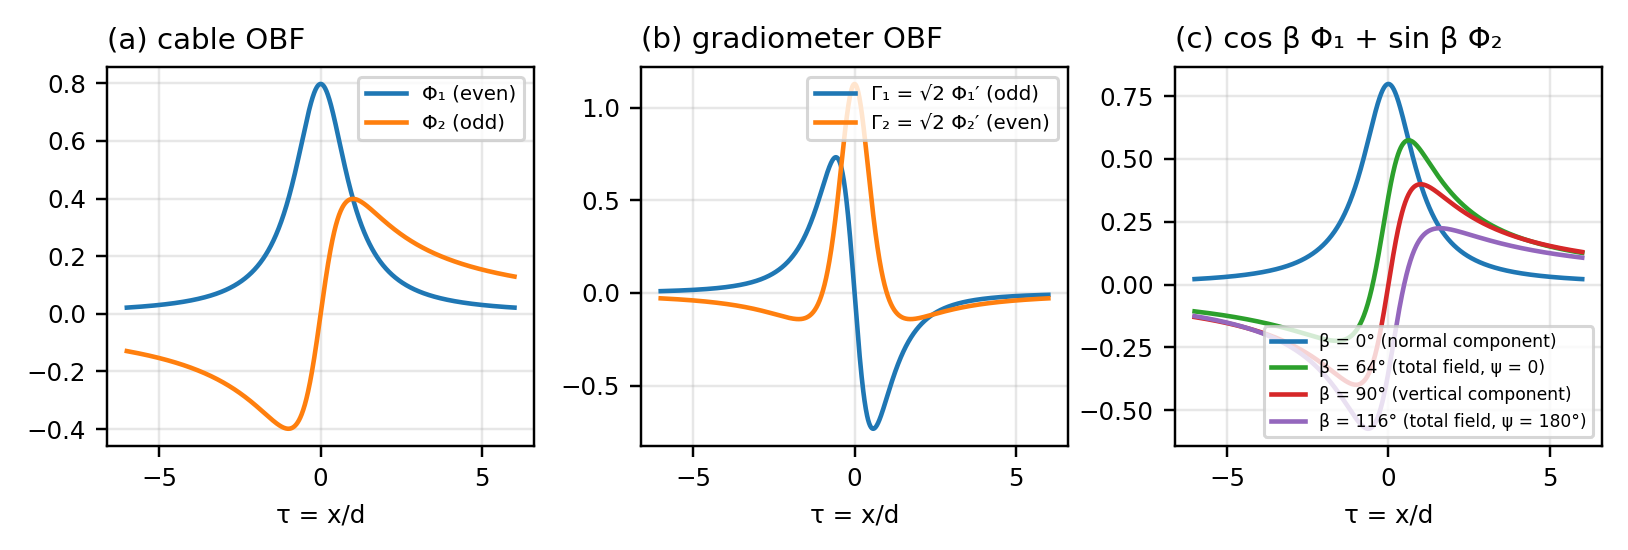
\includegraphics[width=\linewidth]{paper/sec_2_geometry_signal_model/figures/F2_bases.png}
\caption{(a) Cable OBF: the even $\Phi_1$ and the odd $\Phi_2$ of~\eqref{eq:obf}.
(b) Gradiometer OBF: the odd $\Gamma_1$ and the even $\Gamma_2$ of~\eqref{eq:grad_obf}.
(c) Channels of~\eqref{eq:channel} for $\beta = 0^{\circ}$ (normal component), $90^{\circ}$ (vertical component), and the limits $64^{\circ}$ and $116^{\circ}$ of the total-field phase at Brest.}
\label{fig:obf}
\end{figure}